% -*- root: ../main.tex -*-
%modalità di divisione in itinere dei task, meeting/interazioni pianificate, modalità di revisione in itinere dei task, scelta degli strumenti di test/build/continuous integration
\chapter{Processo di Sviluppo} \label{chap:dev-process}
In questo capitolo viene analizzato l'intero processo di sviluppo definito dal team.

\section{Domain Driven Design}
 Fin dall'inizio, è stato scelto un approccio di design fortemente basato sul dominio. Infatti nella discussione preliminare sull'idea, sono emersi molti dubbi sul significato dei vocaboli usati e su concetti generali di funzionamento. Questo ha spinto il team ad avvalersi naturalmente di schemi per chiarificare e uniformare le astrazioni di ogni team-member. Questi schemi sono stati mantenuti e aggiornati per tutta la durata del progetto, uniformando l'artefatto generato con il modello del dominio. Questo permette anche la successiva evoluzione del progetto in modo più semplice.
    \subsection{Aspetti principali}
    I concetti chiave che hanno assunto particolare importanza nello sviluppo sono stati:
    \begin{itemize}
        \item \textbf{Domain Expert interview}: per formalizzare le richieste e non permettere al software di allontanarsi da esse nello sviluppo, l'intervista con l'esperto del dominio è stata formalizzata e trascritta insieme a tutte le domande (capitolo \ref{chap: IntervistaCommittente})
        \item \textbf{Linguaggio Condiviso}: per evitare continue spiegazioni tra i membri del team, per indicare a quale concetto si stesse facendo riferimento, è stata creata una tabella di "Ubiquitous Language" (capitolo \ref{chap:UbiquitousLanguage})
        \item \textbf{User Stories}: per assicurare che l'esperienza sia in linea con quella desiderata e che il software copra ogni interazione utente richiesta, sono state definite tutte le user stories che sono emerse dall'intervista con il committente (capitolo \ref{chap:UserStories})
        \item \textbf{Mockup}: per verificare che il team abbia compreso a pieno l'aspettativa del risultato, sono stati sviluppati dei mockup, che il cliente ha verificato e approvato (capitolo \ref{chap:Mockup})
    \end{itemize}

\section{Metodologia di Sviluppo}
Per sviluppare il progetto è stato scelto il framework \textbf{Scrum}, infatti il processo di sviluppo è stato basato, in comune accordo, sulla metodologia agile. La motivazione risiede nel fatto che il team è composto da quattro persone e il prodotto deve essere sviluppato in tempi brevi. Il framework Scrum infatti permette di suddividere i compiti in modo preciso, sviluppando il progetto in passi incrementali, assicurando di coprire man mano tutti i requisiti richiesti dal cliente.

    \subsection{Scrum}
    Secondo il framework Scrum il lavoro deve essere diviso in più sprint seguendo un approccio iterativo. Per questo motivo l'intervallo di tempo disponibile per lo sviluppo del progetto è stato suddiviso in sotto-intervalli di una settimana. 
    Il team mantiene due tipi di backlog, i quali riflettono l'organizzazione spiegata sopra: il product backlog e lo sprint backlog. 
    
    \paragraph{Product Backlog}Il product backlog racchiude il progresso generale del progetto, in cui ogni item riflette una user-story, o una funzionalità ad alto livello, di cui il cliente può apprezzare lo sviluppo. Queste vengono ordinate per urgenza e dimensione e, scelto un sottoinsieme, assegnate allo sprint successivo. In ogni sprint è presente infatti lo sprint backlog, in cui si può apprezzare l'implementazione più dettagliata e a basso livello delle varie feature. 

    \paragraph{Sprint Backlog} Lo sprint backlog, relativo ad ogni iterazione, va a raffinare nella riunione iniziale (sprint planning) gli item scelti (sprint goal) dal product backlog. Questi sono suddivisi in più task e assegnati a diversi membri del team. Nel meeting finale (sprint review) lo sprint backlog viene ispezionato, riordinato e utilizzato per ulteriori considerazioni sull'iterazione successiva. Per maggiori dettagli sul processo di sviluppo di ogni iterazione si veda il capitolo \ref{chap:Retrospettiva}.

    \paragraph{Definition of done} Un item del product backlog o sprint backlog si ritiene concluso quando tutti i task che lo compongono sono stati completati.
    
    \paragraph{Scrum poker} Per stimare il livello di effort necessario per il completamento di ogni task è stata utilizzata la tecnica che viene chiamata \textbf{scrum poker}. Questa tecnica consiste in una fase preliminare di lettura e discussione di un task e degli aspetti che lo riguardano. Successivamente, ogni membro del team sceglie tra 1, 2, 3, 5, 8, 13, 20 il numero che ritiene più adeguato a rappresentare la complessità del task, ad esempio tenendo conto del tempo ritenuto necessario per lo sviluppo o la difficoltà stimata del task stesso. A seguito della scelta di un numero da parte di ogni membro, vengono rivelati i numeri scelti e si cerca di raggiungere consenso sulla scelta del numero finale, eventualmente argomentando la propria decisione. La scelta del set di numeri da assegnare è tale da avere volutamente ampi intervalli tra i numeri per ridurre conflitti e raggiungere con maggiore semplicità una situazione di consenso.

    \paragraph{Ruoli}
    Dal momento che il team è composto da solo quattro persone, il "domain-expert", lo "scrum master" e il "product owner" hanno preso parte allo sviluppo del progetto anche come programmatori.

\section{Gestione di Progetto}
In questa sezione verrà spiegato come il progetto è stato gestito con diversi tool seguendo la metodologia Scrum.
    \paragraph{Diagramma di Gantt} \label{par:gantt}
    Per l'organizzazione generale del progetto è stato utilizzato un diagramma di Gantt realizzato grazie ai tool forniti da \href{https://www.atlassian.com/software/jira}{Jira}, come si può notare da Figura \ref{fig:jira-start1} e Figura \ref{fig:jira-start2}. Questo ci ha permesso di avere una visione globale dei momenti del progetto e dei task da svolgere in ogni fase. Inoltre, lo strumento è stato utile per monitorare il lavoro svolto nelle varie deadline.

        \begin{figure}[H]
            \centering
            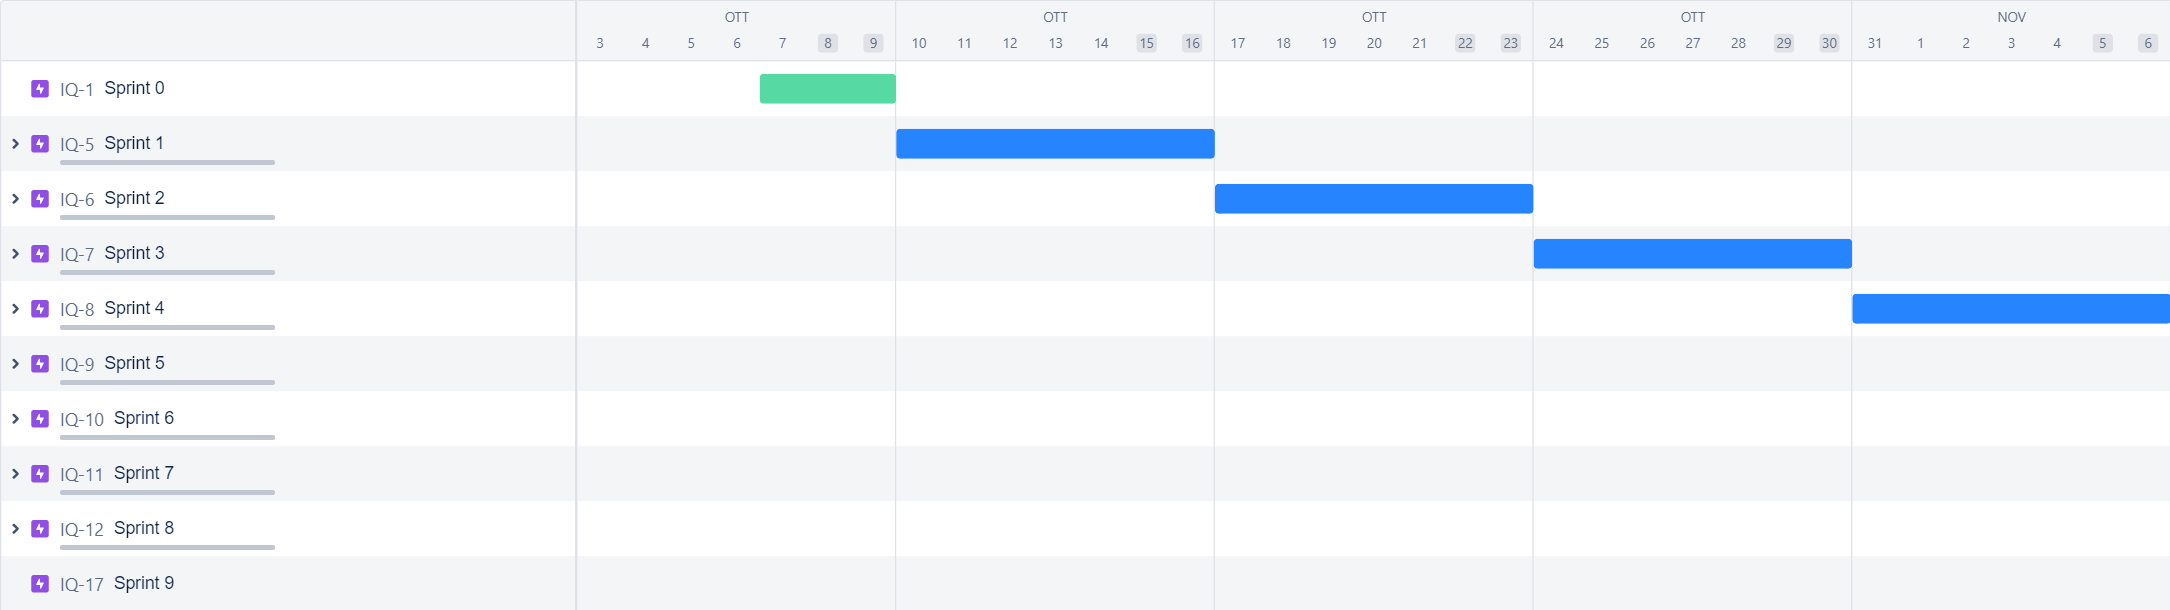
\includegraphics[width=\textwidth]{Images/Jira_sprintInizio1png.png}
            \caption{Diagramma di Gantt all'inizio del processo di sviluppo}
            \label{fig:jira-start1}
        \end{figure}

        \begin{figure}[H]
            \centering
            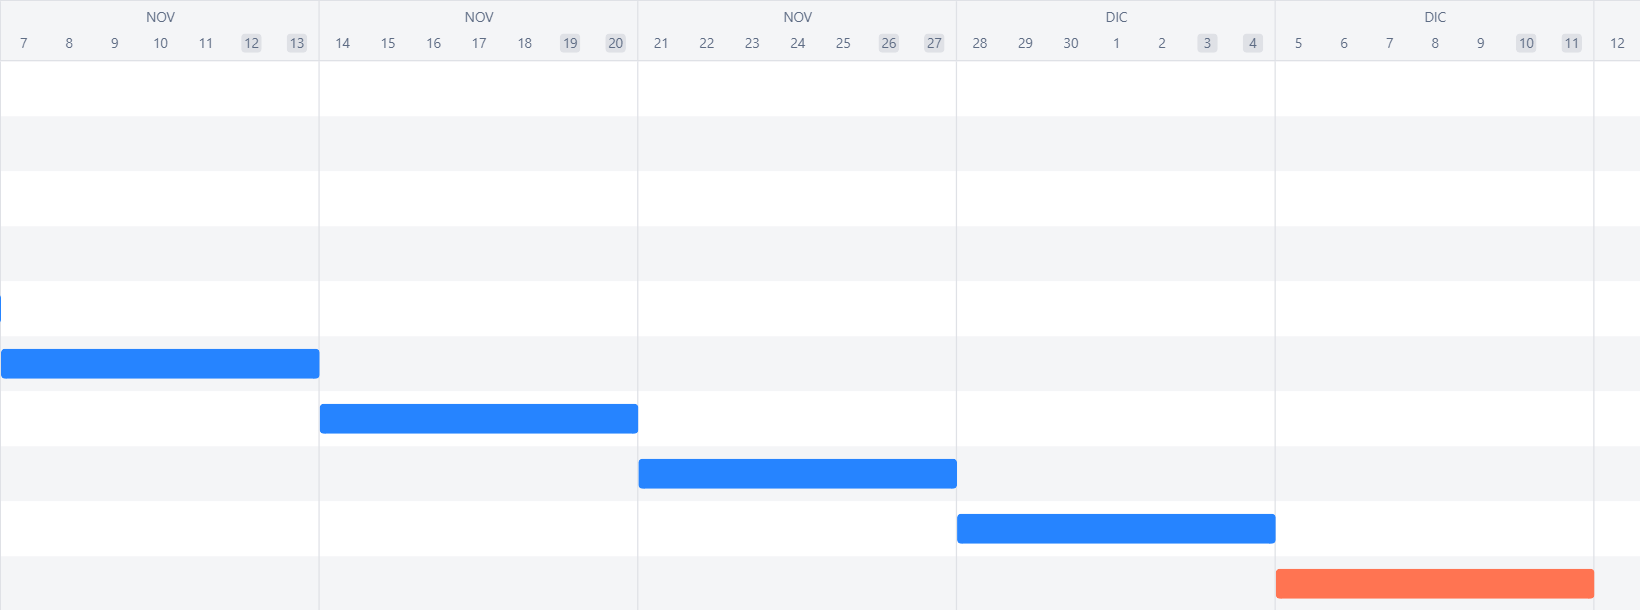
\includegraphics[width=\textwidth]{Images/Jira_sprintInizio2png.png}
            \caption{Diagramma di Gantt all'inizio del processo di sviluppo}
            \label{fig:jira-start2}
        \end{figure}
    
    \paragraph{Collaborative Design Board}
    Per lavorare simultaneamente su grafici e schemi che sono stati molto utili nelle fasi iniziali di analisi e design, è stato utilizzato \href{https://miro.com}{Miro}.

    \paragraph{Product-Backlog} \label{chap:product-backlog}
    Per realizzare le board secondo il framework Scrum è stato utilizzato \href{https://github.com/orgs/ISIQuiz/projects/3}{GitHub-Projects}, un tool che si è rivelato molto potente, grazie anche all'integrazione diretta con \href{https://github.com}{GitHub}. Ad esempio, la chiusura delle issue avviene automaticamente con la merge del relativo branch relativo e gli item corrispondenti vengono spostati correttamente nella board. Inoltre, la possibilità di avere diverse viste sugli stessi dati ha permesso di sviluppare product e sprint backlog senza ripetizioni o duplicazioni. La creazione di diverse view ha permesso anche ai membri del team di osservare facilmente il progresso, la priorità e la grandezza dei task. I vari raffinamenti sono stati referenziati alle issue principali tramite la loro descrizione, in modo da poter osservare il completamento passo passo delle user-stories. Unica mancanza da parte del tool, è quella di non poter assegnare delle issue a più sprint backlog, qualora non venissero completate solamente in uno di essi.
    
    \paragraph{Licensing} 
    Per la licenza è stata scelta \href{https://choosealicense.com/licenses/}{la licenza MIT base}, in quanto il progetto è di natura accademica e non commerciale.
    
    \paragraph{Versioning}
    Riguardo al versioning, la piattaforme scelta è stata \href{https://git-scm.com}{Git}. Dato che il progetto è stato svolto in tempi ristetti, è stato scelto il versioning semantico unito a quello temporale, per cui in ogni versione è presente un'indicazione data da MAJOR.MINOR.PATCH in unione alla data di rilascio.
    
    \paragraph{Git Flow} \label{chap:git-flow}
    Per la gestione del workflow del repository del progetto, è stato utilizzato il modello di branching \textbf{Git Flow} (come schematizzato in Figura \ref{fig:git-flow}). Il branch \textit{main} è stato utilizzato solamente per pubblicare le release del software finito o suoi eventuali aggiornamenti. Il branch \textit{dev} viene invece aggiornato con le versioni stabili di tutte le feature man mano che vengono implementate. Per ogni issue indicata negli sprint backlog, viene creato un branch apposito a partire da \textit{dev}, nel quale verrà implementata la nuova funzionalità per poi essere infine riportata sul branch \textit{dev} una volta terminata.
        \begin{figure}[H]
            \centering
            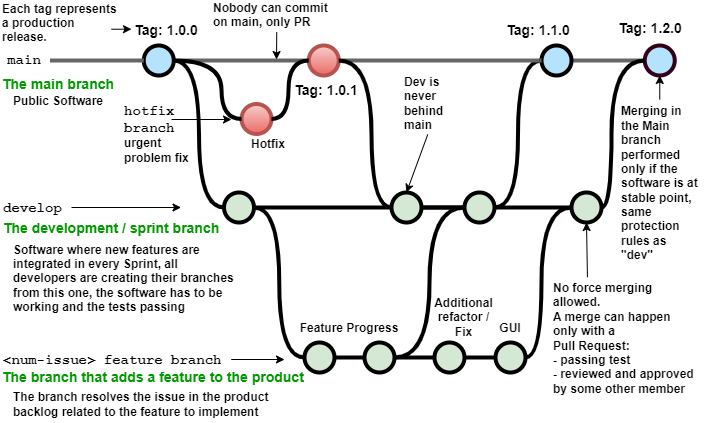
\includegraphics[width=1\textwidth]{Images/git-flow.png}
            \caption{Workflow di Git utilizzato}
            \label{fig:git-flow}
        \end{figure}

    \paragraph{Quality Assurance} \label{chap:QA}
    Per garantire il giusto processo di sviluppo appena indicato, sono state attivate delle \textbf{Branch Protection Rules}. Esse obbligano uno sviluppatore che contribuisce al progetto ad eseguire una pull request prima di poter fare la merge sul branch \textit{dev} del codice da lui implementato nel branch di una feature. 
    Ogni pull request deve ricevere l'approvazione dal almeno uno degli altri membri del progetto e deve anche eseguire correttamente tutti i test automatici presenti nel progetto. Le stesse regole sono state applicate anche quando viene effettuata una release sul branch \textit{main} del codice presente sul branche \textit{dev}.

    \paragraph{Discord}
    \href{https://discord.com}{Discord} è stato utilizzato come strumento di comunicazione vocale per i meeting, per la sua capacità di condividere lo schermo e di supportare chiamate di gruppo. Inoltre, particolarmente utile è stata la divisione delle chat in canali in cui organizzare logicamente il materiale, i link e le discussioni.
    
    \paragraph{Telegram}
    La scelta di \href{https://telegram.org}{Telegram} come strumento di comunicazione informale è motivata dal fatto che dispone di funzionalità avanzate orientate ai programmatori e che tutti i membri del gruppo la utilizzano personalmente come applicazione di messaggistica.
    
    \paragraph{Telegram Bot} 
    Per mantenere tutti i membri aggiornati sul progresso del progetto, è stato creato ed inserito nel gruppo Telegram un Bot. Tale Bot è stato utilizzato per notificare ogni richiesta di review di una pull request e ciascun caricamento di una nuova versione del report.
    Dato l'elevato tempo necessario alla CI per terminare il processo di generazione del PDF del report o del sito web del progetto, le notifiche del Bot sono state utili per verificare l'esito di tali operazioni una volta portate a termine.

\section{Continuous Integration e Automatizzazione}\label{chap:CI}
Nel progetto la Continuous Integration (CI) e l'automatizzazione delle mansioni più ripetitive hanno avuto notevole importanza. Una cospicua quantità di tempo è stata dedicata all'inizio per la messa in opera di pipeline che permettano di risparmiare tempo successivamente agli sviluppatori e di garantire la massima qualità al cliente finale.
    \subsection{Report}
        I tool utilizzati per la CI del report sono:
        \begin{itemize}
            \item \href{https://www.latex-project.org/}{\LaTeX}
            \item \href{https://www.overleaf.com/}{Overleaf}
            \item \href{https://github.com/features/actions}{GitHub Actions}
            \item \href{https://core.telegram.org/bots/api}{Telegram Bots}
            \item \href{https://pandoc.org/}{Pandoc}
            \item \href{https://pages.github.com/}{GitHub Pages}
        \end{itemize}
        
        \paragraph{\LaTeX}La relazione di progetto è stata svolta in \LaTeX. Questa decisione è motivata dal fatto che esso permette facilmente di organizzare lunghi testi in capitoli e sottocapitoli, eventualmente riordinando intere parti senza preoccuparsi dell'indice o della formattazione. Inoltre, permette la gestione in maniera più accurata, rispetto al Markdown, di elementi grafici, tabelle, stili, link e referenze, producendo un PDF finale di qualità elevata.
        
        \paragraph{Overleaf}
        Come strumento complementare è stato scelto Overleaf, una piattaforma che permette la collaborazione ininterrottamente e simultanea sullo stesso blocco di testo. Questo è risultato utile nella produzione dei documenti relativi agli "Sprint-planning" e, sopratutto, durante gli "Sprint-review".
        
        \paragraph{GitHub-Actions}
        Per la Continuous Integration, sono state sfruttate a pieno le GitHub-Actions messe a disposizione da GitHub. Queste permettono di generare il PDF finale in automatico e di renderlo pubblico con Release istantanee ad ogni cambiamento. Ciò ha non solo alleviato la preoccupazione di farlo manualmente, ma ha anche permesso di rendere disponibile al cliente sempre l'ultima versione aggiornata. 
        
        \paragraph{Bot Telegram}
        Per garantire la massima qualità, un Bot Telegram è stato utilizzato come strumento di notifica nel gruppo Telegram dedicato. Il Bot notifica, come in Figura \ref{fig:CI-Report}, qualora ci sia qualunque problema in ogni step della CI o, in caso di successo, avverte che l'azione è stata portata a termine correttamente ed inoltra il PDF sul gruppo.
            \begin{figure}[H]
                \centering
                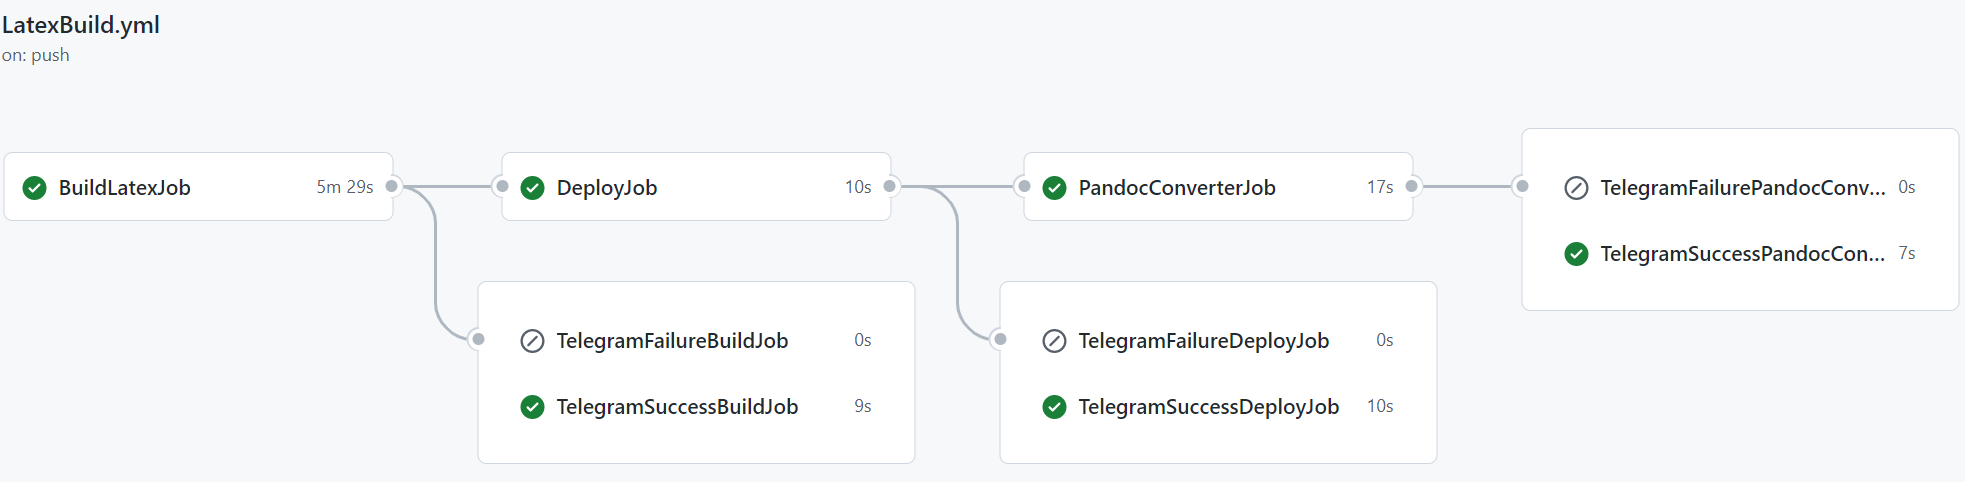
\includegraphics[width=1\textwidth]{Images/CI-Report.png}
                \caption{Pipeline Continuous Integration per il report}
                \label{fig:CI-Report}
            \end{figure}

        \paragraph{Pandoc}
        Qualora una persona volesse consultare la relazione online, senza scaricare il PDF, si è fatto uso di Pandoc per generare il relativo sito web consultabile direttamente sul browser. Per la paginazione, è stato utilizzato un template HTML/CSS per rendere la vista più accattivante.
        
        \paragraph{GitHub-Pages}
        Per il deploy del sito è stato utilizzato GitHub-Pages che permette di semplificarne la messa in opera avendo un branch dedicato sul quale tutti i file relativi possono essere mantenuti e aggiornati.

    \subsection{Progetto Software}
        I tool utilizzati per la CI del software sono:
        \begin{itemize}
            \item Sbt 1.7.2
            \item ScalaTest 3.2.14
            \item Sbt-assembly 2.0.0
            \item GitHub Actions
            \item \href{https://github.com/orgs/ISIQuiz/projects/3}{GitHub Boards}
            \item GitHub Pages
            \item Dependabot
            \item ScalaDoc
            \item ScalaCoverage
            \item Telegram Bots
            \item Sonarcloud/Codacy/Codefactor
            \item Jira
            \item Miro
            \item \href{https://www.planitpoker.com}{PlanItPoker}
        \end{itemize}
        
        Per quanto riguarda la Continuous Integration del software, come prima cosa è stato fatto il setup dello \textbf{Scala Build Tool}, specificando la versione di scala da utilizzare nel progetto, la versione di sbt stesso, inserendo le dipendenze di scalatest e il plugin sbt-assembly negli appositi file di configurazione. In modo analogo alla relazione, sono state poi utilizzate le \textbf{GitHub-Actions} per automatizzare la verifica dei test e per la release dei jar eseguibili. In particolare, ad ogni commit, i test vengono eseguiti nella \textbf{GitHub-Actions} bloccando, in caso di fallimento, la merge sugli altri branch. Nel caso in cui sia possibile eseguire il merge di una pull request, viene inviato un messaggio sul gruppo Telegram, grazie a \textbf{GitHub-Actions} e \textbf{Telegram-bot}, che notifica l'avvenuta risoluzione del task e la necessità di una review.
        
        \begin{figure}[H]
            \centering
            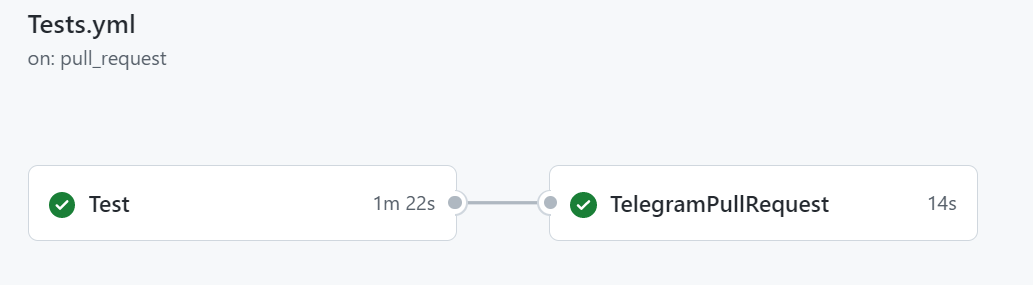
\includegraphics[width=0.8\textwidth]{Images/CI-Test-PR.png}
            \caption{Pipeline per l'esecuzione dei test e la notifica di una pull request}
            \label{fig:CI-Test-PR}
        \end{figure}

        Nel caso in cui una pull request venga correttamente chiusa portando il codice sviluppato sul branch \textit{dev}, la issue relativa alla feature implementata viene automaticamente chiusa su \textbf{GitHubBoards}. La Continuous Integration è stata utilizzata anche per generare la pagina principale del sito web del software, dove sono presenti i link al report, alla coverage e alla documentazione del software realizzata tramite \textbf{ScalaDoc}. Per automatizzare il processo di deploy del sito web è stato utilizzato \textbf{GitHub-Pages}, mentre per generare la parte relativa al riepilogo dei test è stato usato \textbf{ScalaCoverage}.
            \begin{figure}[H]
                \centering
                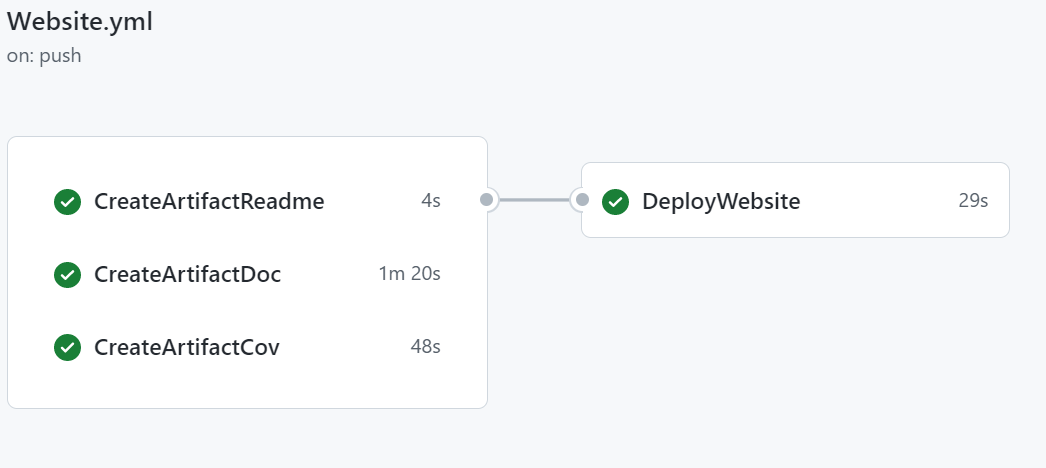
\includegraphics[width=0.8\textwidth]{Images/CI-Website.png}
                \caption{Pipeline per il deploy del sito web}
                \label{CI-Website}
            \end{figure}
        
        Per le release del software è stata realizzata una pipeline eseguita ogni volta che delle funzionalità vengono spostate dal branch \textit{dev} al branch \textit{main}.
        Tale pipilene è strutturata in modo tale da eseguire tutti i test e generare lo \textit{uber jar} (ovvero un \textit{jar} contenente tutte le dipendenze e le risorse necessarie per l'esecuzione indipendente) in caso di completo successo dei test. Per la creazione del jar eseguibile è stato utilizzato \textbf{Sbt-assembly} e viene automaticamente caricato tra nelle release del progetto.
        
            \begin{figure}[H]
                \centering
                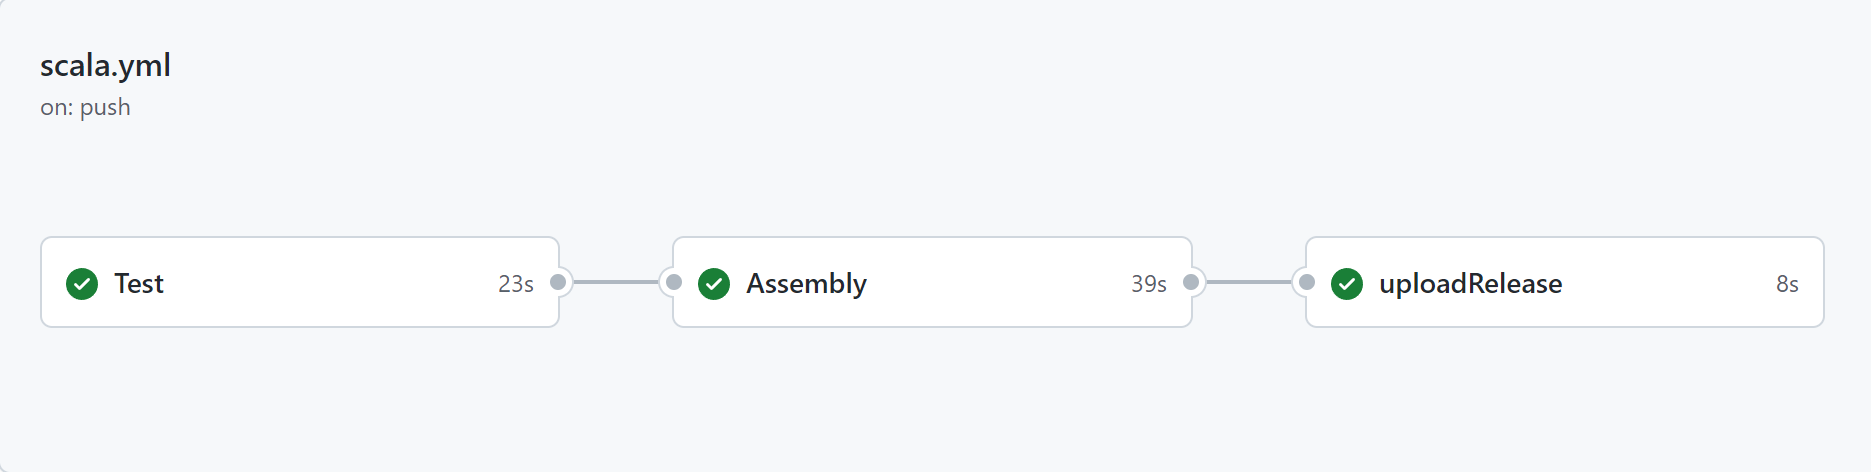
\includegraphics[width=1\textwidth]{Images/CI-Test-Deploy.png}
                \caption{Pipeline per il deploy delle release}
                \label{fig:CI-Test-Deploy}
            \end{figure}  

